\documentclass[crop,tikz]{standalone}
\begin{document}
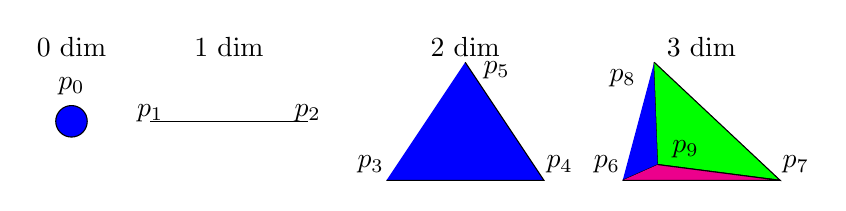
\begin{tikzpicture}
  \draw[fill=blue] (0,.75) circle (0.2);
  \draw (0,1.2) node{ $p_0$};
  \draw (0,1.7) node{0 dim};

  \draw (1,.75) -- (3,.75);
  \draw (1,.85) node{$p_1$};
  \draw (3,.85) node{$p_2$};
  \draw (2,1.7) node{1 dim};

  \draw[fill=blue] (4,0) -- (6,0) -- (5,1.5);
  \draw (3.8,.2) node{$p_3$};
  \draw (6.2,.2) node{$p_4$};
  \draw (5.4,1.4) node{$p_5$};
  \draw (5,1.7) node{2 dim};

  \draw[fill=blue] (7,0) -- (7.45,.2) -- (7.4,1.5);
  \draw[fill=green] (7.45,.2) -- (9,0) -- (7.4,1.5);
  \draw[fill=magenta] (7,0) -- (9,0) -- (7.45,.2);
  \draw (6.8,.2) node{$p_6$};
  \draw (9.2,.2) node{$p_7$};
  \draw (7,1.3) node{$p_8$};
  \draw (7.8,.4) node{$p_9$};
  \draw (8,1.7) node{3 dim};
\end{tikzpicture}
\end{document}
